\documentclass{article}

\usepackage{graphicx}
\usepackage{hyperref}
\usepackage{apacite}

\title{MAS ISW Assignment 4}
\date{30.11.2020}
\author{Simon Deussen}

\begin{document}
  \pagenumbering{gobble}
  \maketitle
  \pagenumbering{arabic}

  \section*{Task 6: Create a one page summary of two given papers}
  \subsection*{Summary: \emph{How to Read an Engineering Research Paper}}
  
  In the given paper \cite{griswold2009read}, the author suggests several tips on how two
  effectively read a research paper. He starts by encouraging the reader and then begins with analyzing  
  the structure of typical research paper. Following items are mentioned:
  \begin{itemize}
    \item Abstract
    \item Introduction
    \item Related work 
    \item Background
    \item System or model
    \item Contribution
    \item Performance or evaluation
    \item Conclusions
    \item References.
  \end{itemize}

  The author emphasizes to read the paper out of order and to start with the important parts like Abstract, 
  Introduction, Contribution and Conclusion. One of the key things he suggested is a series of eight question 
  a reader should be able to answer after reading or skimming through a research paper. After reading a paper,
  the reader should ideally immediately annotate it with answers to those question as well as key take aways.
  \begin{enumerate}
    \item What are \emph{motivations} for this work?
    \item What is the proposed \emph{solution}?
    \item What is the work`s \emph{evaluation} of the proposed solution?
    \item What is your analysis of the identified problam,idea and evaluation?
    \item What are the \emph{contributions}?
    \item What are \emph{future directions} for this research? 
    \item What questions are you left with?
    \item What is the main take away message of  this paper?
  \end{enumerate}
A suggestion is to use a standard form for every paper to keep track of the own thoughts and to be fast able to 
find ideas again. Another important point to remember is to check the papers context.
For this it is important to find out if the read paper classifies as a generalization of a topic, if its a
new research direction or if its contradicts existing research.
Further the author suggest to read everything twice, first to get a general big picture of the content and a second
time to get all the details.
He wraps up the guide with the important question: \emph{Are you convinced that the paper proposed a viable solution?}

\subsection*{Summary: \emph{How to read a research paper}}

This paper \cite{Huang} is a similar how-to about effective paper reading.
The authors first writes about where to get papers. He mentioned two main sources: conferences and archival journals. The 
difference between them is the length of the content. Conference papers tend to be shorter and newer and journal paper are longer 
and stronger reviewed writes the author.

Further he recommends those specific sources for research in robotics:  
\begin{itemize}
  \item IEEE Transactions on Robotics and Automation
  \item International Journal of Robotics Research
  \item Autonomous Robots
  \item IEEE Conference on Robotics and Automation (ICRA)
  \item IEEE/RSJ Conference on Robots and Systems (IROS)
\end{itemize}

As a next thing he suggests citeseer and google scholar for discovering papers. The last two sections are quite similar to the first one
\cite{griswold2009read}. The first section contains question the reader should answer after reading the paper, and the second contains
tips for the order of the read sections.
\begin{itemize}
  \item What problems are they solving?
  \item What did they really do?
  \item What is the contribution?
  \item What methods did they use? 
  \item Would you have solved the problem differently?
  \item Do all pieces fit together logically?
  \item What were the results? Did they do what they set out to do?
\end{itemize}
One of the final tips if the author is to point out how important the references are if you want to research yourself, because 
they will point to similar work worth studying.

% \begin{figure}[h!]
%   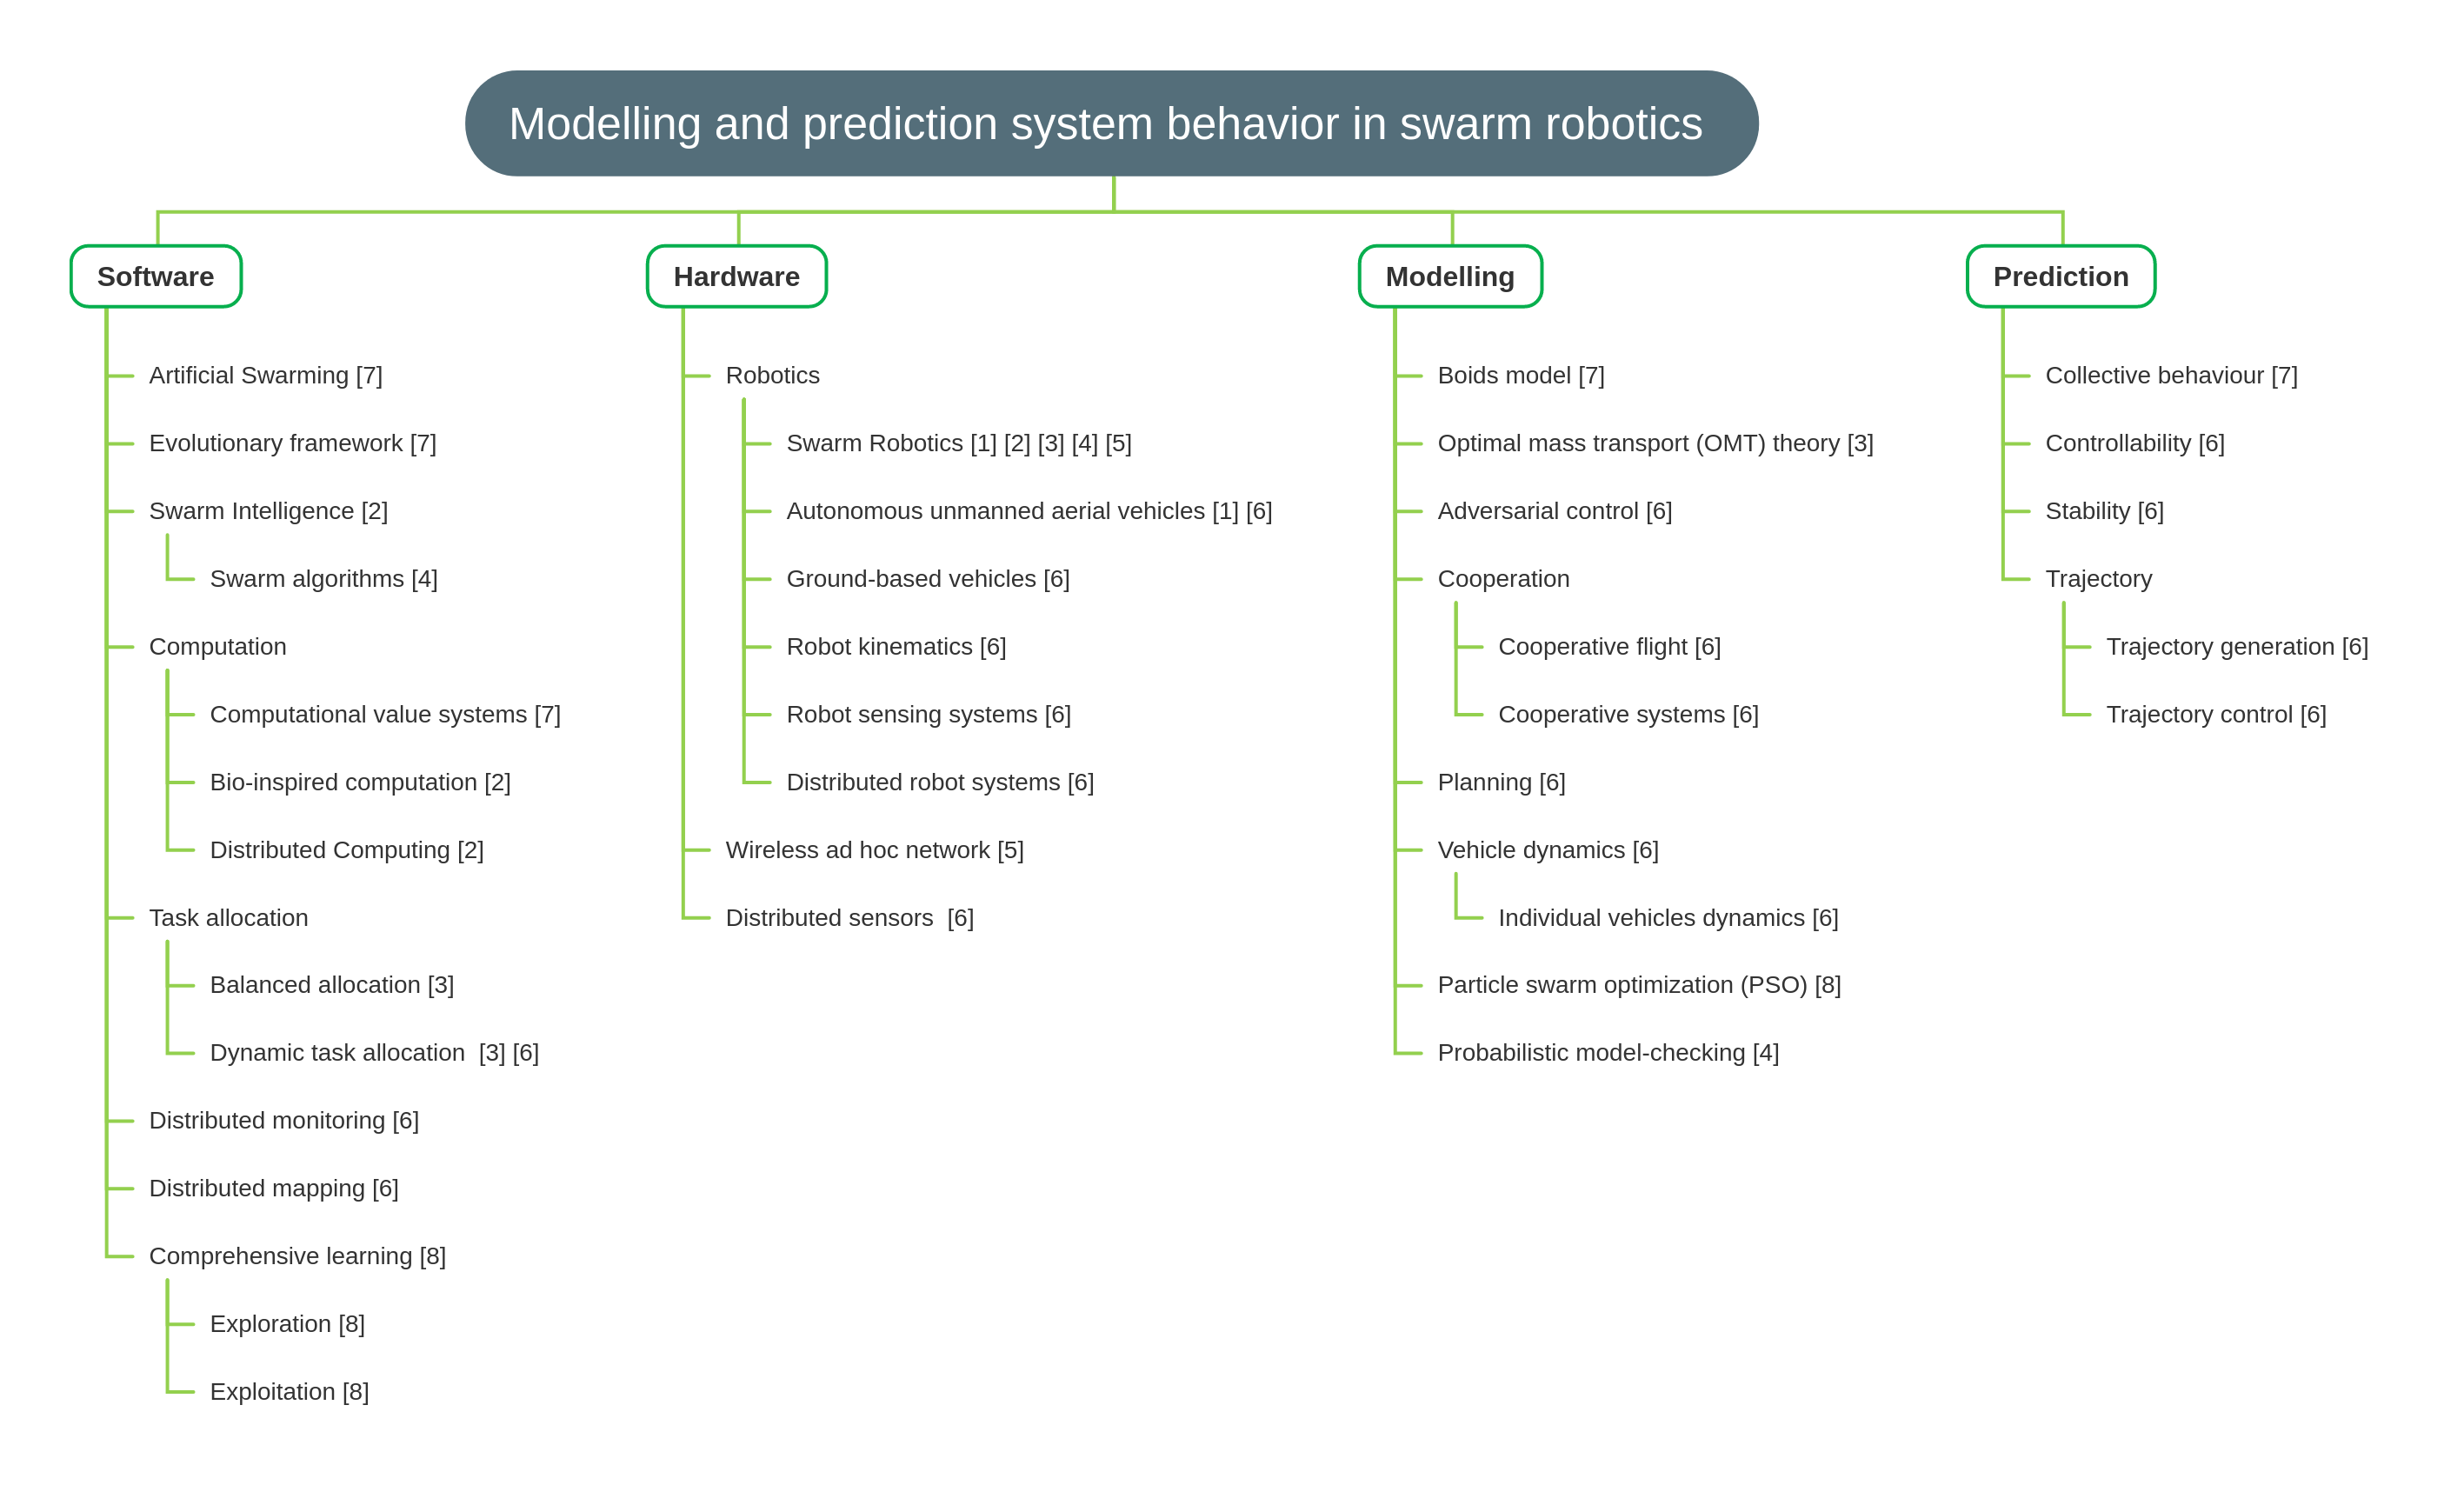
\includegraphics[width=\linewidth]{Robotics.png}
%   \caption{Mindmap of the keywords.}
%   \label{fig:rob}
% \end{figure}

\bibliography{stuff}
\bibliographystyle{apacite}

\end{document}